% Copyright (C) 2005 Thomas L. Kula
% All Rights Reserved
%
% See the file LICENSE for license terms.
\documentclass[12pt]{article}
\usepackage{graphicx}
\setlength{\paperwidth}{5.5in}
\setlength{\paperheight}{8.5in}
\setlength{\textheight}{6.45in}
\setlength{\oddsidemargin}{-0.5in}
\setlength{\evensidemargin}{-0.5in}
\setlength{\textwidth}{4.0in}
\setlength{\parindent}{0in}
\setlength{\parskip}{3mm}
\usepackage[print]{booklet} \nofiles
\source{\magstep0}{5.5in}{8.5in}
\target{\magstep0}{11in}{8.5in}
\setpdftargetpages
\begin{document}


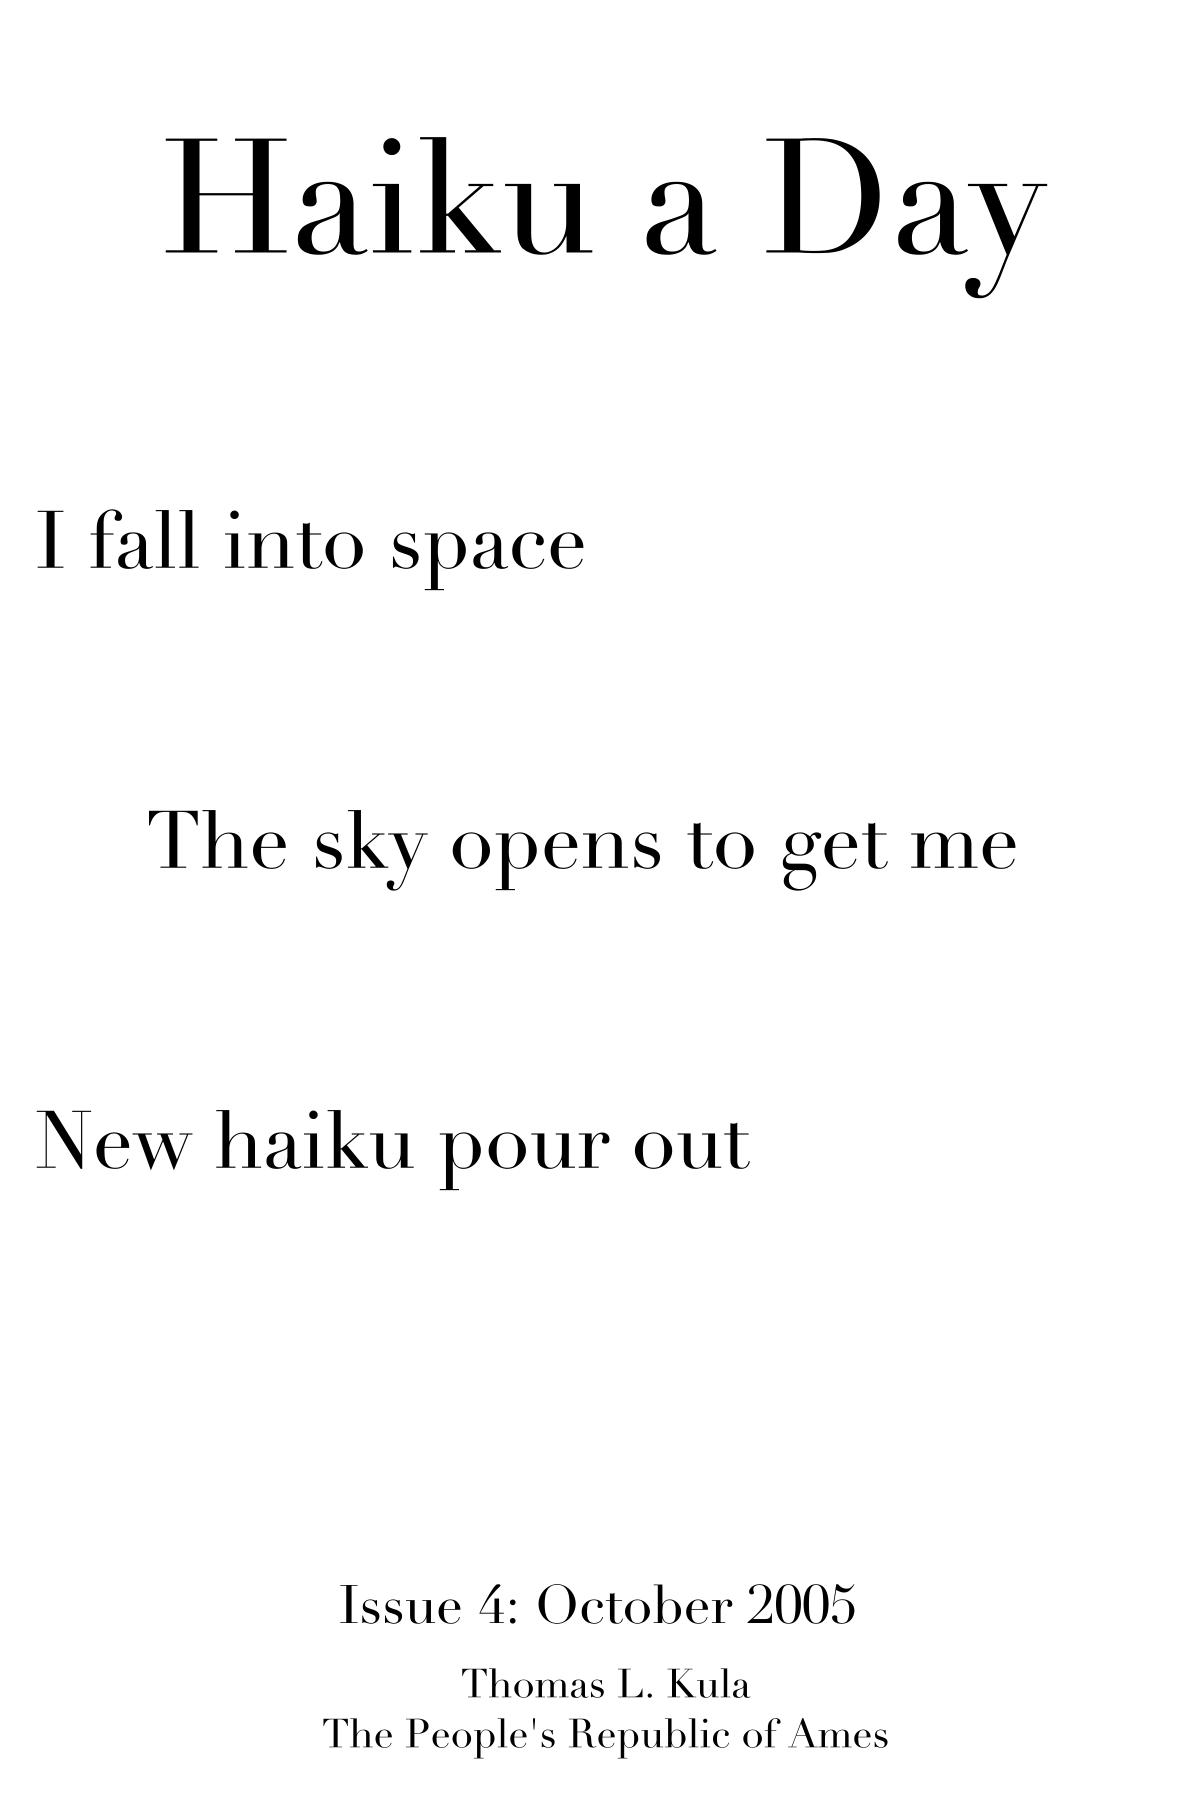
\includegraphics[width=101mm]{frontpage.png}

\newpage

Hey, we've made it to the third month. That's a quarter year.
Spiffy.

Next month I'm participating in the National Novel Writing
Month --- {\tt http://www.nanowrimo.org/ } --- at least,
if I can come up with a plot before November. 50000 words,
30 days, not a problem, right?


Enjoy.

--- Thomas

P.O. Box 1124 \\
Ames, IA 50014-1124 \\
http://kula.tproa.net/had/

Downloadable version available at website, or if you really
want me to send you one, send me your address, maybe a
stamp too.

\newpage
\setlength{\parskip}{1mm}

1 September 2005

Motorcycles blare \\
Loud noises zip down the street \\
I hate those damn things \\

2 September 2005

Books placed everywhere \\
Stuffed wherever they could fit \\
A shelf full  of joy \\

3 September 2005

Ugh, fucking raisins \\
You looked like cranberries there \\
Now my muffin sucks \\


4 September 2005

Dry garbonzo beans \\
Look like tiny little brains \\
Much loved by zombies \\

5 September 2005

The Day of Labor \\
We gave to you the weekend. \\
Long live the Wobblies \\

6 September 2005

Tea in a plain mug \\
Not as neat as a tea set \\
I guess it will do \\

\newpage

7 September 2005 

Paintings on the wall \\
Some are cool, some are not so \\
All are someone's work \\

8 September 2005

Sky dark, day is night \\
A ferocious storm blows through \\
Mother Nature wakes. \\

9 September 2005

Football tomorrow \\
Drunken morons fill the streets \\
Why am I in town? \\


10 September 2005

Water glass moisture \\
Condensation in the heat \\
Muggy night outside \\

11 September 2005

Battle's Barbeque \\
Your sign still says Blimpies Subs \\
Update it perhaps? \\

12 September 2005

History Majors \\
But not cool ones, stupid ones \\
Mouth diarrhea \\

\newpage

13 September 2005

Stuffed grape leaves are good \\
I should learn how to make them \\
And not get from can. \\

14 September 2005

Bundled newspapers \\
A stack there for recycling \\
Yellow and musty \\

15 September 2005

A clean living room \\
It rarely happens to me \\
But I enjoy it \\


16 September 2005 

Sweater weather starts \\
Leaves start falling to the ground \\
Fall peeks into Ames \\

17 September 2005

A mass exodus \\
Raindrops falling from the sky \\
Now I sit inside. \\

18 September 2005

Back tire was fixed \\
But blew out on north Hyland \\
So buy a spare tube \\

\newpage

19 September 2005

Black plaid black great kilt \\
As dark as my blighted soul \\
Perfect for curling \\

20 September 2005

Clear starry fall night \\
Each star so big yet so small \\
I am but a speck \\

21 September 2005

Curling injury \\
A sore sholder all day long \\
It's lame but it hurts \\


22 September 2005

Salada green tea \\
Sucks so much it's not funny \\
Throw that box away \\

23 September 2005

Late night vendo land \\
Tasty snacks, comforting lights \\
Screw you, nutrition! \\

24 September 2005

Broasted potatoes \\
Someone somewhere is eating \\
Now I am hungry \\

\newpage

25 September 2005

Table after rain \\
Drops of water speckle it \\
Now my butt is wet \\

26 September 2005

Things to think about: \\
Seven-Eleven chopsticks \\
Why do these exist? \\

27 September 2005

Fire engines howl \\
Racing past me down the street \\
Into the fire \\


28 September 2005

Free junk food at work \\
Temptingly there, so I eat \\
Now my tummy hurts \\

29 September 2005

Happy organ songs \\
Sweet music in a dim room \\
Mates of State are good \\

30 September 2005

To make a pencil: \\
Think of all the stuff you need \\
And the stuff it needs \\


\newpage


\includegraphics[width=101mm]{backpage.png}

\end{document}




